\section{Data}
\label{sec:data}

\subsection{Dataset Construction}

Daily log-returns for the SPY ETF are downloaded via \texttt{yfinance} and stored
locally in \texttt{data/df\_sp\_500\_log\_ret.csv}. The raw return on day $t$ is
defined as
\[
  r_t = \ln\!\left(\frac{P_t}{P_{t-1}}\right),
\]
where $P_t$ denotes the adjusted closing price. A sliding-window dataset is then
constructed with a look-back of $L \geq 10$ lags:
\begin{align*}
  X_t &= (r_{t-1},\, r_{t-2},\, \ldots,\, r_{t-L}) \in \mathbb{R}^{L}, \\
  y_t &= \sigma_t \in \mathbb{R}_{+},
\end{align*}
where $\sigma_t$ is the realized absolute return (rolling standard deviation of returns
over a short window), serving as a proxy for next-day volatility.

\subsection{Descriptive Statistics}

Table~\ref{tab:stats} reports summary statistics for the full sample.

\begin{table}[H]
  \centering
  \caption{Descriptive statistics for S\&P 500 daily log-returns (SPY, 1993--2026).}
  \label{tab:stats}
  \begin{tabular}{lr}
    \toprule
    Statistic & Value \\
    \midrule
    Observations  & 8\,343 \\
    Start date    & 1993-02-01 \\
    End date      & 2026-03-24 \\
    Mean          & $0.0004$ \\
    Std deviation & $0.0117$ \\
    Minimum       & $-0.1159$ \\
    Maximum       & $+0.1356$ \\
    Skewness      & $-0.248$ \\
    Kurtosis      & $11.42$ \\
    \bottomrule
  \end{tabular}
\end{table}

The distribution exhibits \textbf{negative skewness} (large negative shocks more common
than large positive ones) and \textbf{excess kurtosis} of 11.42, confirming heavy tails
relative to a Gaussian distribution. Both features are consistent with the well-known
stylised facts of equity returns.

\subsection{Log-Return Time Series}

\begin{figure}[H]
  \centering
  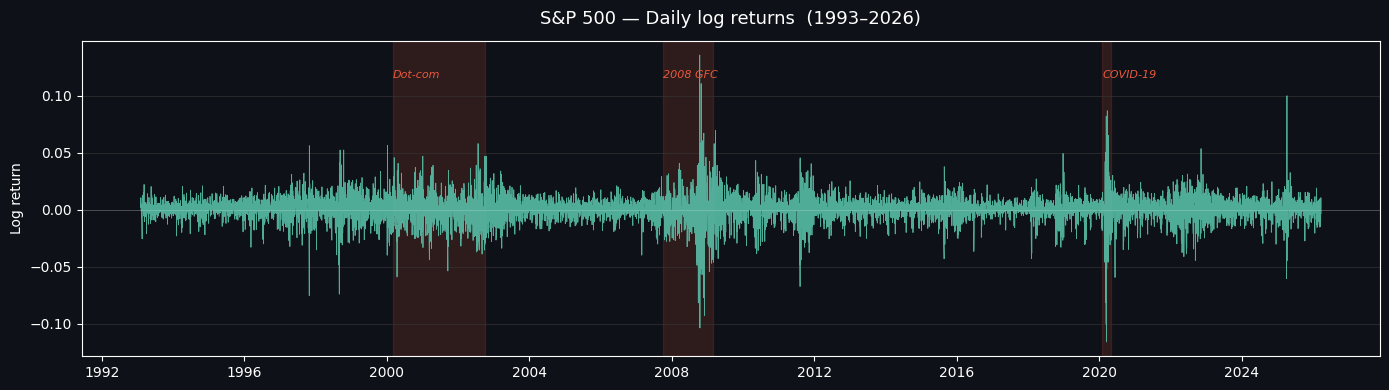
\includegraphics[width=\textwidth]{figures/figure_21.png}
  \caption{S\&P 500 daily log-returns. Three major stress periods are clearly visible.}
  \label{fig:log_returns}
\end{figure}

Returns oscillate around zero with no discernible trend, consistent with the
efficient market hypothesis. Three major stress episodes are visible: the dot-com crash
(2000--2002), the Global Financial Crisis (2008--2009), and the COVID shock (2020).
These episodes exhibit the characteristic feature of \textbf{volatility clustering}: large
moves arrive in bursts and calm periods are interspersed.

\subsection{Realized Volatility and Regime Identification}

\begin{figure}[H]
  \centering
  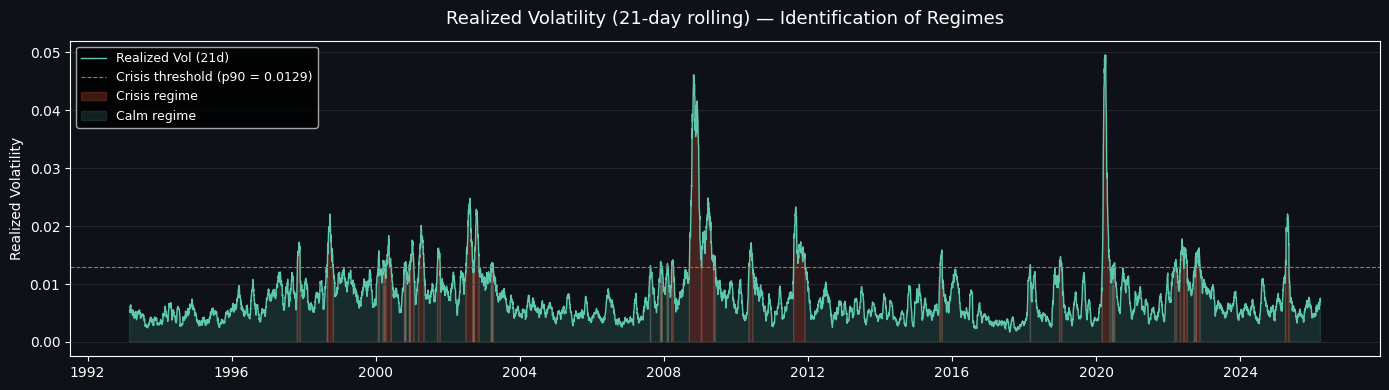
\includegraphics[width=\textwidth]{figures/figure_22.png}
  \caption{Realized absolute return (target variable $y_t$). The dashed line indicates
    the 90th-percentile threshold used to define the crisis regime.}
  \label{fig:realized_vol}
\end{figure}

A threshold at the \textbf{90th percentile} ($\sigma^* = 1.117$) is used to split the
sample into two regimes:

\begin{table}[H]
  \centering
  \caption{Market regime statistics.}
  \label{tab:regimes}
  \begin{tabular}{lrr}
    \toprule
    Regime  & Share of observations & Characterization \\
    \midrule
    Calm    & 90\%  & Low, stable volatility \\
    Crisis  & 10\%  & Sharp spikes; three major episodes \\
    \bottomrule
  \end{tabular}
\end{table}

The pronounced asymmetry in regime frequency is critical: a model that performs well on
average may still fail badly during the 10\% of days that matter most for risk management.

\subsection{Autocorrelation Analysis}

\begin{figure}[H]
  \centering
  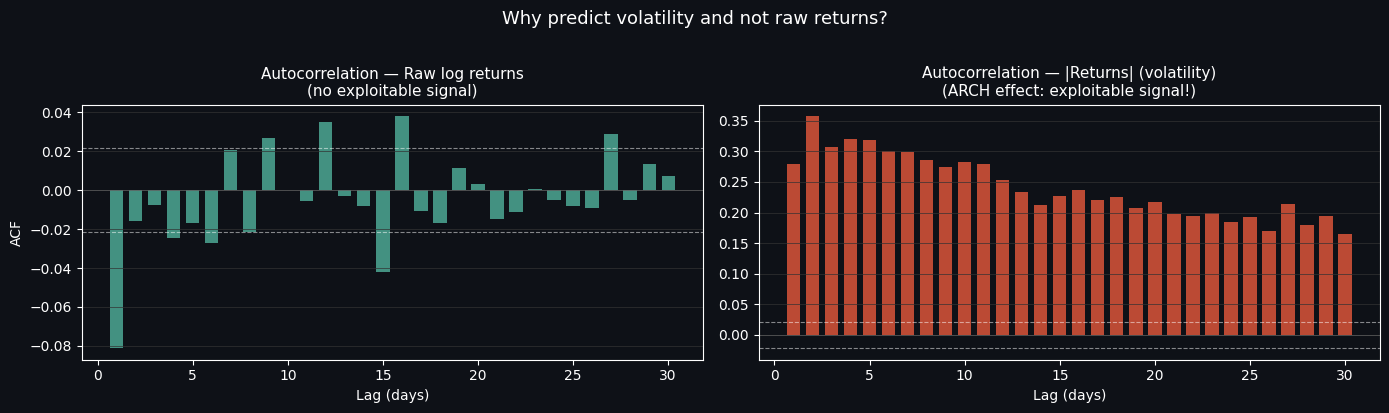
\includegraphics[width=\textwidth]{figures/figure_23.png}
  \caption{Autocorrelation of raw log-returns (near zero) vs absolute log-returns
    (strongly positive). The latter justifies using past absolute returns as features.}
  \label{fig:acf}
\end{figure}

Two key findings:
\begin{itemize}
  \item \textbf{Raw log-returns}: autocorrelation is essentially zero at all lags ---
        the return series itself is unpredictable.
  \item \textbf{Absolute log-returns / realized volatility}: autocorrelation is
        strongly and persistently positive (the ARCH effect), justifying the use of past
        lagged returns as features for predicting future volatility.
\end{itemize}

\subsection{Feature Correlation Structure}

\begin{figure}[H]
  \centering
  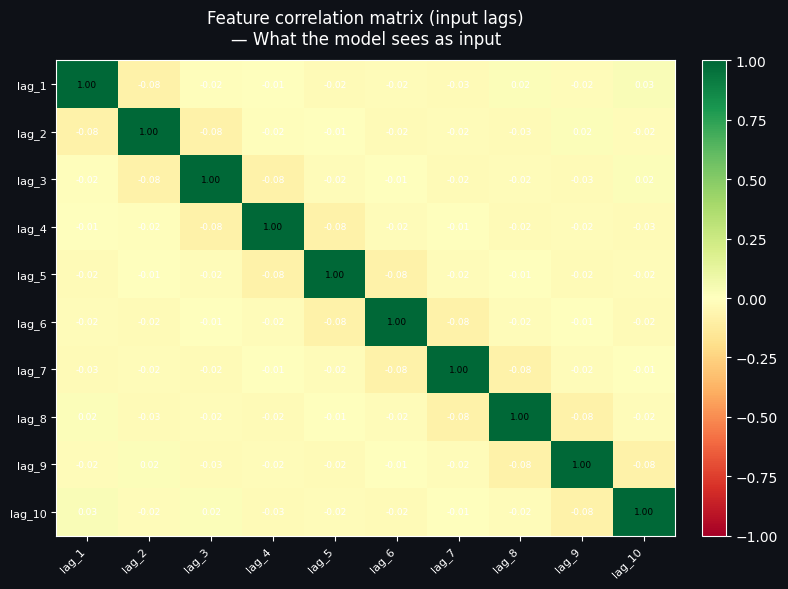
\includegraphics[width=\textwidth]{figures/figure_24.png}
  \caption{Pearson correlation matrix of the 10 lag features. Adjacent lags are
    positively correlated, reflecting the persistence of volatility regimes.}
  \label{fig:corr}
\end{figure}

Adjacent lags are positively correlated due to volatility clustering: a large move on
day $t-1$ is likely to be followed by a large move on day $t-2$. This introduces mild
multicollinearity for linear models and gives sequential models such as the RNN a structural
advantage.

\subsection{Summary}

Three statistical properties of the data guide the modelling choices throughout this
report:
\begin{enumerate}
  \item \textbf{Raw returns are unpredictable} (near-zero ACF) --- the target must be
        the magnitude, not the sign, of returns.
  \item \textbf{Volatility is autocorrelated} (ARCH effect) --- past lags carry genuine
        predictive information.
  \item \textbf{Two regimes coexist} --- calm and crisis periods have fundamentally
        different statistical properties; a good model must handle both.
\end{enumerate}
